\section{\RU{Глобальные переменные}\EN{Global variables}}
\index{\RU{Глобальные переменные}\EN{Global variables}}
\label{scanf_global_variable}

\RU{А что если переменная \TT{x} из предыдущего примера будет глобальной переменной, а не локальной? 
Тогда к ней смогут обращаться из любого другого места, а не только из тела функции. 
Глобальные переменные считаются \glslink{anti-pattern}{анти-паттерном},
но ради примера мы можем себе это позволить.}
\EN{What if the \TT{x} variable from the previous example was not local but a global one? 
Then it would have been accessible from any point, not only from the function body. 
Global variables are considered \gls{anti-pattern}, but for the sake of the experiment, we could do this.}

\lstinputlisting{patterns/04_scanf/2_global/ex2.c.\LANG}

\subsection{MSVC: x86}

\lstinputlisting{patterns/04_scanf/2_global/ex2_MSVC.asm}

\RU{В целом ничего особенного. Теперь \TT{x} объявлена в сегменте \TT{\_DATA}. 
Память для неё в стеке более не выделяется.
Все обращения к ней происходит не через стек, а уже напрямую. 
Неинициализированные глобальные переменные не занимают места в исполняемом файле
(и действительно, зачем в исполняемом файле
нужно выделять место под изначально нулевые переменные?), но тогда, когда к этому месту в памяти
кто-то обратится, \ac{OS} подставит туда блок, состоящий из нулей\footnote{Так работает \ac{VM}}.}
\EN{In this case the \TT{x} variable is defined in the \TT{\_DATA} segment and no memory is allocated in the local stack. It is accessed directly, not through the stack. 
Uninitialized global variables take no space in the executable file
(indeed, why one needs to allocate space for variables initially set to zero?), 
but when someone accesses their address, 
the \ac{OS} will allocate a block of zeroes there\footnote{That is how a \ac{VM} behaves}.}

\RU{Попробуем изменить объявление этой переменной:}
\EN{Now let's explicitly assign a value to the variable:}

\lstinputlisting{patterns/04_scanf/2_global/default_value.c.\LANG}

\RU{Выйдет в итоге:}\EN{We got:}

\begin{lstlisting}
_DATA	SEGMENT
_x	DD	0aH

...
\end{lstlisting}

\RU{Здесь уже по месту этой переменной записано \TT{0xA} с типом DD (dword = 32 бита).}
\EN{Here we see a value \TT{0xA} of DWORD type (DD stands for DWORD = 32 bit) for this variable.}

\RU{Если вы откроете скомпилированный .exe-файл в \IDA, то увидите, что \IT{x} 
находится в начале сегмента \TT{\_DATA}, после этой переменной будут текстовые строки.}
\EN{If you open the compiled .exe in \IDA, you can see the \IT{x} variable placed at the beginning of 
the \TT{\_DATA} segment, and after it you can see text strings.}

\RU{А вот если вы откроете в \IDA .exe скомпилированный в прошлом примере, 
где значение \IT{x} не определено, то вы увидите:}
\EN{If you open the compiled .exe from the previous example in \IDA, where the value of \IT{x} was not
set, you would see something like this:}

\begin{lstlisting}
.data:0040FA80 _x              dd ?                    ; DATA XREF: _main+10
.data:0040FA80                                         ; _main+22
.data:0040FA84 dword_40FA84    dd ?                    ; DATA XREF: _memset+1E
.data:0040FA84                                         ; unknown_libname_1+28
.data:0040FA88 dword_40FA88    dd ?                    ; DATA XREF: ___sbh_find_block+5
.data:0040FA88                                         ; ___sbh_free_block+2BC
.data:0040FA8C ; LPVOID lpMem
.data:0040FA8C lpMem           dd ?                    ; DATA XREF: ___sbh_find_block+B
.data:0040FA8C                                         ; ___sbh_free_block+2CA
.data:0040FA90 dword_40FA90    dd ?                    ; DATA XREF: _V6_HeapAlloc+13
.data:0040FA90                                         ; __calloc_impl+72
.data:0040FA94 dword_40FA94    dd ?                    ; DATA XREF: ___sbh_free_block+2FE
\end{lstlisting}

\RU{\TT{\_x} обозначен как \TT{?}, наряду с другими переменными не требующими инициализации. 
Это означает, что при загрузке .exe в память, место под всё это выделено будет и будет заполнено
нулевыми байтами \cite[6.7.8p10]{C99TC3}. 
Но в самом .exe ничего этого нет. Неинициализированные переменные не занимают места в исполняемых файлах. 
Это удобно для больших массивов, например.}
\EN{\TT{\_x} is marked with \TT{?} with the rest of the variables that do not need to be initialized. 
This implies that after loading the .exe to the memory, a space for all these variables is to be 
allocated and filled with zeroes \cite[6.7.8p10]{C99TC3}. 
But in the .exe file these uninitialized variables do not occupy anything.
This is convenient for large arrays, for example.}

\ifdefined\IncludeOlly
\clearpage
\subsection{MSVC: x86 + \olly}
\index{\olly}

\RU{Тут даже проще}\EN{Things are even simpler here}:

\begin{figure}[H]
\centering
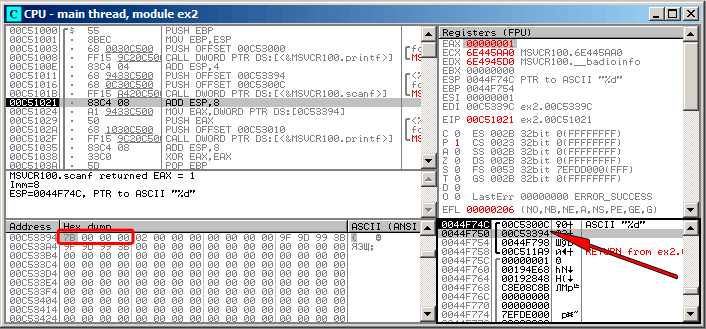
\includegraphics[scale=\FigScale]{patterns/04_scanf/2_global/ex2_olly_1.png}
\caption{\olly: \RU{после исполнения \scanf}\EN{after \scanf execution}}
\label{fig:scanf_ex2_olly_1}
\end{figure}

\RU{Переменная хранится в сегменте данных.}
\EN{The variable is located in the data segment.}
\RU{Кстати, после исполнения инструкции \PUSH (заталкивающей адрес $x$) адрес появится в стеке, 
и на этом элементе можно нажать правой кнопкой, выбрать \q{Follow in dump}.}
\EN{After the \PUSH instruction (pushing the address of $x$) gets executed, 
the address appears in the stack window. Right-click on that row and select \q{Follow in dump}.}
\RU{И в окне памяти слева появится эта переменная.}
\EN{The variable will appear in the memory window on the left.}

\RU{После того как в консоли введем 123, здесь появится}\EN{After we have entered 123 in the console,} 
\TT{0x7B}\EN{ appears in the memory window (see the highlighted screenshot regions)}.

\RU{Почему самый первый байт это}\EN{But why is the first byte} \TT{7B}?
\RU{По логике вещей, здесь должно было бы быть}\EN{Thinking logically,} \TT{00 00 00 7B}\EN{ should be
there}.
\RU{Это называется}\EN{The cause for this is referred as } \gls{endianness}, \RU{и в x86 принят формат }\EN{and x86 uses }\IT{little-endian}.
\RU{Это означает, что в начале записывается самый младший байт, а заканчивается самым старшим байтом}%
\EN{This implies that the lowest byte is written first, and the highest written last}.
\RU{Больше об этом}\EN{Read more about it at}: \myref{sec:endianness}.

\RU{Позже из этого места в памяти 32-битное значение загружается в \EAX и передается в}
\EN{Back to the example, the 32-bit value is loaded from this memory address into \EAX and passed to} \printf.

\RU{Адрес переменной $x$ в памяти}\EN{The memory address of $x$ is} \TT{0x00C53394}.

\clearpage
\RU{В \olly{} мы можем посмотреть карту памяти процесса (Alt-M) и увидим, что этот адрес
внутри PE-сегмента \TT{.data} нашей программы}%
\EN{In \olly we can review the process memory map (Alt-M)
and we can see that this address is inside the \TT{.data} PE-segment of our program}:

\begin{figure}[H]
\centering
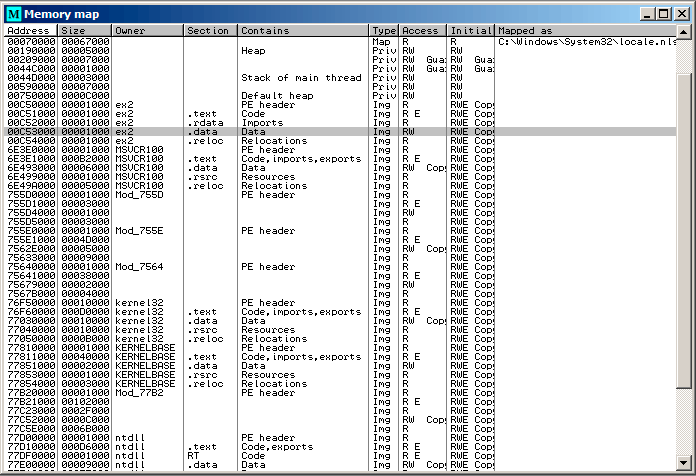
\includegraphics[scale=\FigScale]{patterns/04_scanf/2_global/ex2_olly_2.png}
\caption{\olly: \RU{карта памяти процесса}\EN{process memory map}}
\label{fig:scanf_ex2_olly_2}
\end{figure}

\fi

\ifdefined\IncludeGCC
\subsection{GCC: x86}

\index{ELF}
\RU{В Linux всё почти также. За исключением того, что если значение \TT{x} не определено, 
то эта переменная будет находится в сегменте \TT{\_bss}.
В \ac{ELF} этот сегмент имеет такие атрибуты:}
\EN{The picture in Linux is near the same, with the difference that the uninitialized variables are located in the \TT{\_bss} segment. 
In \ac{ELF} file this segment has the following attributes:}

\begin{lstlisting}
; Segment type: Uninitialized
; Segment permissions: Read/Write
\end{lstlisting}

\RU{Ну а если сделать статическое присвоение этой переменной какого-либо
значения, например, 10, то она будет находится 
в сегменте \TT{\_data},
это сегмент с такими атрибутами:}
\EN{If you, however, initialise the variable with some value e.g. 10, 
it is to be placed in the \TT{\_data} segment, which has the following attributes:}

\begin{lstlisting}
; Segment type: Pure data
; Segment permissions: Read/Write
\end{lstlisting}
\fi

\subsection{MSVC: x64}

\lstinputlisting[caption=MSVC 2012 x64]{patterns/04_scanf/2_global/ex2_MSVC_x64.asm.\LANG}

\RU{Почти такой же код как и в}\EN{The code is almost the same as in} x86.
\RU{Обратите внимание что для \TT{scanf()} адрес переменной $x$ передается
при помощи инструкции \LEA, а во второй \printf передается само значение переменной при помощи \MOV}
\EN{Please note that the address of the $x$ variable is passed to \TT{scanf()} using a \LEA instruction,
while the variable's value is passed to the second \printf using a \MOV instruction}.
\TT{DWORD PTR}\RU{\EMDASH{}это часть языка ассемблера (не имеющая отношения к машинным кодам) 
показывающая, что тип переменной в памяти именно 32-битный, 
и инструкция \MOV должна быть здесь закодирована соответственно}\EN{ is a part of the assembly language (no relation to the machine code), indicating that the variable data size is 32-bit and the \MOV instruction
has to be encoded accordingly}.

\ifdefined\IncludeARM
\subsection{ARM: \OptimizingKeilVI (\ThumbMode)}

\begin{lstlisting}
.text:00000000 ; Segment type: Pure code
.text:00000000                 AREA .text, CODE
...
.text:00000000 main
.text:00000000                 PUSH    {R4,LR}
.text:00000002                 ADR     R0, aEnterX     ; "Enter X:\n"
.text:00000004                 BL      __2printf
.text:00000008                 LDR     R1, =x
.text:0000000A                 ADR     R0, aD          ; "%d"
.text:0000000C                 BL      __0scanf
.text:00000010                 LDR     R0, =x
.text:00000012                 LDR     R1, [R0]
.text:00000014                 ADR     R0, aYouEnteredD___ ; "You entered %d...\n"
.text:00000016                 BL      __2printf
.text:0000001A                 MOVS    R0, #0
.text:0000001C                 POP     {R4,PC}
...
.text:00000020 aEnterX         DCB "Enter X:",0xA,0    ; DATA XREF: main+2
.text:0000002A                 DCB    0
.text:0000002B                 DCB    0
.text:0000002C off_2C          DCD x                   ; DATA XREF: main+8
.text:0000002C                                         ; main+10
.text:00000030 aD              DCB "%d",0              ; DATA XREF: main+A
.text:00000033                 DCB    0
.text:00000034 aYouEnteredD___ DCB "You entered %d...",0xA,0 ; DATA XREF: main+14
.text:00000047                 DCB 0
.text:00000047 ; .text         ends
.text:00000047
...
.data:00000048 ; Segment type: Pure data
.data:00000048                 AREA .data, DATA
.data:00000048                 ; ORG 0x48
.data:00000048                 EXPORT x
.data:00000048 x               DCD 0xA                 ; DATA XREF: main+8
.data:00000048                                         ; main+10
.data:00000048 ; .data         ends
\end{lstlisting}

\RU{Итак, переменная \TT{x} теперь глобальная, и она расположена, почему-то, в другом сегменте, а именно сегменте данных}
\EN{So, the \TT{x} variable is now global and for this reason located in another segment, namely the data segment} (\IT{.data}).
\RU{Можно спросить, почему текстовые строки расположены в сегменте кода (\IT{.text}), а \TT{x} нельзя было разместить тут же?}
\EN{One could ask, why are the text strings located in the code segment (\IT{.text}) and \TT{x} is located right here?}
\RU{Потому что эта переменная, и как следует из определения, она может меняться. И может быть, меняться часто.}
\EN{Because it is a variable and by definition its value could change. Moreover it could possibly change often.}
\RU{Ну а текстовые строки имеют тип констант, они не будут меняться, поэтому они располагаются в сегменте \IT{.text}.}
\EN{While text strings has constant type, they will not be changed, so they are located in the \IT{.text} segment.}
\index{\RAM}
\index{\ROM}
\RU{Сегмент кода иногда может быть расположен в ПЗУ микроконтроллера (не забывайте, 
мы сейчас имеем дело с embedded-микроэлектроникой, где дефицит памяти~--- обычное дело),
а изменяемые переменные~--- в ОЗУ.}
\EN{The code segment might sometimes be located in a \ac{ROM} chip (remember, we now deal
with embedded microelectronics, and memory scarcity is common here), and changeable 
variables~---in \ac{RAM}.}
\RU{Хранить в ОЗУ неизменяемые данные, когда в наличии есть ПЗУ, не экономно.}
\EN{It is not very economical to store constant variables in RAM when you have ROM.}
\RU{К тому же, сегмент данных в ОЗУ с константами нужно инициализировать перед работой,
ведь, после включения ОЗУ, очевидно, она содержит в себе случайную информацию.}
\EN{Furthermore, constant variables in RAM must be initialized, because after powering on, the RAM, obviously, contains random information.}

\index{\RU{Компоновщик}\EN{Linker}}
\RU{Далее мы видим в сегменте кода хранится указатель на переменную \TT{x} (\TT{off\_2C}) и 
все операции с переменной происходят через этот указатель.}
\EN{Moving forward, we see a pointer to the \TT{x} (\TT{off\_2C}) variable in the code segment, and that all
operations with the variable occur via this pointer.}
\RU{Это связано с тем, что переменная \TT{x} может быть расположена где-то довольно далеко от 
данного участка кода, так что её адрес нужно сохранить в непосредственной близости к этому коду.}
\EN{That is because the \TT{x} variable could be located somewhere far from this particular code fragment, so its address
must be saved somewhere in close proximity to the code.}
\index{ARM!\Instructions!LDR}
\RU{Инструкция \TT{LDR} в Thumb-режиме может адресовать только переменные в пределах вплоть 
до 1020 байт от своего местоположения.}
\EN{The \TT{LDR} instruction in Thumb mode can only address variables in a range of 1020 bytes from its location, }
\RU{Эта же инструкция в ARM-режиме~--- переменные в пределах $\pm{}4095$ байт.}
\EN{and in in ARM-mode~---variables in range of $\pm{}4095$ bytes.}
\RU{Таким образом,
адрес глобальной переменной \TT{x} нужно расположить в непосредственной близости, ведь нет никакой гарантии, 
что компоновщик\footnote{linker в англоязычной литературе} сможет разместить саму переменную где-то рядом, 
она может быть даже в другом чипе памяти!}
\EN{And so the address of the \TT{x} variable
must be located somewhere in close proximity, because there is no guarantee that the linker would be able to accommodate the variable somewhere nearby the code, it may well be even in an external memory chip!}

\index{\CLanguageElements!const}
\index{\ROM}
\RU{Ещё одна вещь: если переменную объявить как \IT{const}, то компилятор Keil разместит её в 
сегменте \TT{.constdata}.}
\EN{One more thing: if a variable is declared as \IT{const}, the Keil compiler allocates it in 
the \TT{.constdata} segment.}
\RU{Должно быть, впоследствии компоновщик и этот сегмент сможет разместить в ПЗУ вместе
с сегментом кода.}
\EN{Perhaps, thereafter, the linker could place this segment in ROM too, along with the code segment.}

\subsection{ARM64}

\lstinputlisting[caption=\NonOptimizing GCC 4.9.1 ARM64,numbers=left]{patterns/04_scanf/2_global/ARM64_GCC491_O0.s.\LANG}

\index{ARM!\Instructions!ADRP/ADD pair}
\RU{Теперь $x$ это глобальная переменная, и её адрес вычисляется при помощи пары инструкций ADRP/ADD 
(строки 21 и 25).}
\EN{In this case the $x$ variable is declared as global and its address is calculated using 
the ADRP/ADD instruction pair (lines 21 and 25).}

\fi
\ifdefined\IncludeMIPS
\subsection{MIPS}

\subsubsection{\EN{Uninitialized global variable}\RU{Неинициализированная глобальная переменная}}

\RU{Так что теперь переменная $x$ глобальная.}
\EN{So now the $x$ variable is global.}
\RU{Сделаем исполняемый файл вместо объектного и загрузим его в \IDA.}
\EN{Let's compile to executable file rather than object file and load it into \IDA.}
\RU{IDA показывает присутствие переменной $x$ в ELF-секции .sbss (помните о \q{Global Pointer}? \myref{MIPS_GP}),
так как переменная не инициализируется в самом начале.}
\EN{IDA displays the $x$ variable in the .sbss ELF section (remember the \q{Global Pointer}? \myref{MIPS_GP}),
since the variable is not initialized at the start.}

\lstinputlisting[caption=\Optimizing GCC 4.4.5 (IDA)]{patterns/04_scanf/2_global/MIPS/O3_IDA.lst.\LANG}

\RU{IDA уменьшает количество информации, так что сделаем также листинг используя objdump и добавим туда свои комментарии:}%
\EN{IDA reduces the amount of information, so we'll also do a listing using objdump and comment it:}

\lstinputlisting[caption=\Optimizing GCC 4.4.5 (objdump),numbers=left]{patterns/04_scanf/2_global/MIPS/O3_objdump.txt.\LANG}

\RU{Теперь мы видим, как адрес переменной $x$ берется из буфера 64KiB, используя GP и прибавление
к нему отрицательного смещения (строка 18).}
\EN{Now we see the $x$ variable address is read from a 64KiB data buffer using GP and adding
negative offset to it (line 18).}
\RU{И даже более того: адреса трех внешних функций, используемых в нашем примере (\puts, \scanf, \printf)
также берутся из буфера 64KiB используя GP (строки 9, 16 и 26).}
\EN{More than that, the addresses of the three external functions  which are used in our example (\puts, \scanf, \printf), are also read from the 64KiB global data buffer using GP (lines 9, 16 and 26).}
\RU{GP указывает на середину буфера, так что такие смещения могут нам подсказать, что адреса всех трех функций,
а также адрес переменной $x$ расположены где-то в самом начале буфера.}
\EN{GP points to the middle of the buffer, and such offset suggests that all three function's addresses,
and also the address of the $x$ variable, are all stored somewhere at the beginning of that buffer.}
\RU{Действительно, ведь наш пример крохотный}\EN{That make sense, because our example is tiny}.

\index{MIPS!\Pseudoinstructions!MOVE}
\index{MIPS!\Pseudoinstructions!NOP}
\RU{Ещё нужно отметить что функция заканчивается двумя \ac{NOP}-ами (\TT{MOVE \$AT,\$AT}~--- 
это холостая инструкция), чтобы выровнять начало следующей функции по 16-байтной границе.}
\EN{Another thing worth mentioning is that the function ends with two \ac{NOP}s (\TT{MOVE \$AT,\$AT} --- 
an idle instruction), in order to align next function's start on 16-byte boundary.}

\subsubsection{\RU{Инициализированная глобальная переменная}\EN{Initialized global variable}}

\RU{Немного изменим наш пример и сделаем, чтобы у $x$ было значение по умолчанию:}
\EN{Let's alter our example by giving the $x$ variable a default value:}

\lstinputlisting{patterns/04_scanf/2_global/default_value.c.\LANG}

\RU{Теперь IDA показывает что переменная $x$ располагается в секции .data:}
\EN{Now IDA shows that the $x$ variable is residing in the .data section:}

\lstinputlisting[caption=\Optimizing GCC 4.4.5 (IDA)]{patterns/04_scanf/2_global/MIPS/O3_IDA_init.lst.\LANG}

\RU{Почему не .sdata? Может быть, нужно было указать какую-то опцию в GCC?}
\EN{Why not .sdata? Perhaps that this depends on some GCC option?}
\RU{Тем не менее, $x$ теперь в .data, а это уже общая память и мы можем посмотреть как происходит
работа с переменными там.}
\EN{Nevertheless, now $x$ is in .data, which is a general memory area, and we can take a look
how to work with variables there.}

\index{MIPS!\Instructions!LUI}
\index{MIPS!\Instructions!ADDIU}
\RU{Адрес переменной должен быть сформирован парой инструкций.}
\EN{The variable's address must be formed using a pair of instructions.}
\RU{В нашем случае это LUI (\q{Load Upper Immediate}~--- загрузить старшие 16 бит) и 
ADDIU (\q{Add Immediate Unsigned Word}~--- прибавить значение).}
\EN{In our case those are LUI (\q{Load Upper Immediate}) and ADDIU (\q{Add Immediate Unsigned Word}).}

\RU{Вот так же листинг сгенерированный objdump-ом для лучшего рассмотрения:}
\EN{Here is also the objdump listing for close inspection:}

\lstinputlisting[caption=\Optimizing GCC 4.4.5 (objdump)]{patterns/04_scanf/2_global/MIPS/O3_objdump_init.txt.\LANG}

\index{MIPS!\Instructions!LUI}
\index{MIPS!\Instructions!ADDIU}
\index{MIPS!\Instructions!LW}
\RU{Адрес формируется используя LUI и ADDIU, но старшая часть адреса
всё ещё в регистре \$S0, и можно закодировать смещение в инструкции LW (\q{Load Word}), так что одной
LW достаточно для загрузки значения из переменной и передачи его в \printf.}
\EN{We see that the address is formed using LUI and ADDIU, but the high part of address is still in
the \$S0 register, and it is possible to encode the offset in a LW (\q{Load Word}) instruction, so one single LW is enough 
to load a value from the variable and pass it to \printf.}

\RU{Регистры хранящие временные данные имеют префикс T-, но здесь есть также регистры с префиксом S-,
содержимое которых должно быть сохранено в других функциях (т.е. \q{saved}).}
\EN{Registers holding temporary data are prefixed with T-, but here we also see some prefixed with S-, 
the contents of which is need to be preserved before use in other functions (i.e., \q{saved}).}
% FIXME:
% This needs to be clarified a bit, e.g. "the registers need to be preserved if a function is called and it wants to use them
\RU{Вот почему \$S0 был установлен по адресу 0x4006cc и затем был использован по адресу 0x4006e8
после вызова \scanf.}
\EN{That is why the value of \$S0 was set at address 0x4006cc and was used again
at address 0x4006e8, after the \scanf call. }
\RU{Функция \scanf не изменяет это значение.}\EN{The \scanf function does not change its value.}

% TODO non-optimized example?

\fi
